%priprava posamezne ure
%tukaj zaporedoma napisemo{st. zaporedne ure}{datum}{naslov}{poglavje}{oblika dela}{pripomocki}
\begin{priprava}{}{}{Integral}{Vrtenine}{frontalna}{tabla}

Če funkcijo $ f(x) $, ki je na $ [a, b] $ enakega predznaka, zavrtimo za $ 360° $ okoli $ x $-osi, dobimo \emph{rotacijsko telo} ali \emph{vrtenino} \didopomba{Mogoče kakšen aplet, ki v živo prikazuje rotacijo in dobljen plašč?}.

\begin{figure*}[h!]
    \centering
    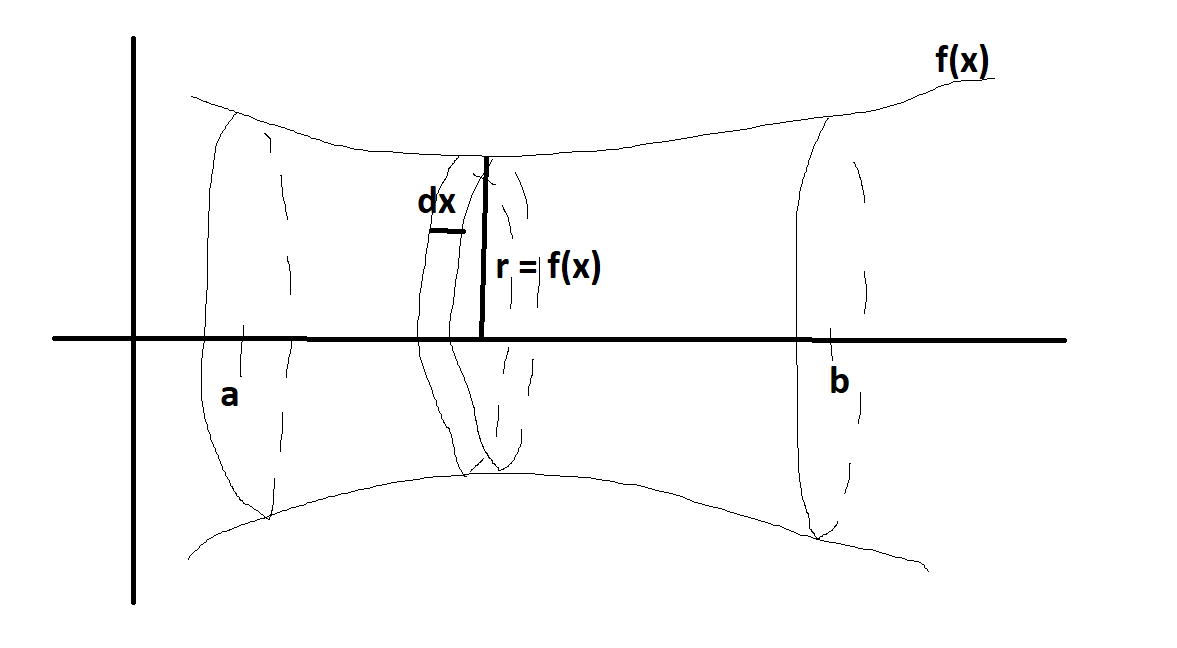
\includegraphics[width=0.6\textwidth]{slike/volumen_vrtenine.png}
\end{figure*}
    
Dobljeno vrtenino narežemo \didopomba{Kot salamco. Naj čimveč sami ugotovijo} na tanke kolobarje/valje (presek je krog). Vsak mali valj ima prostornino $ \pi r^2 \cdot dx = \pi f^2(x) dx $. Gledamo vse $ x $-e na $ [a, b] $, zato za celoten volumen vzamemo integral \didopomba{enak princip kot pri ploščini}:

$$ V = \int_a^b \pi f^2(x) dx = \pi \int_a^b f^2(x) dx $$

\vaje{
Vaje:
\begin{itemize}
    \item \didopomba{Naj sami predlagajo funckije!} Volumen krogle ( $ x^2 + y^2 = r^2 $, integriraš na $ [0, r] $ in pomnožiš z 2), valja ($ y = r $ na $ [0, v] $ ), stožca ($ y = \frac{r}{v} x $ na $ [0, v] $), elipsoida ($ \frac{x^2}{a^2} + \frac{y^2}{b^2} = 1 \rightarrow \frac{4 \pi a b^2}{3} $)
    \item $ y = \sqrt{x}, [0, 3] $
    \item Območje, ki ga nad $ x $-osjo omejujeta funkciji $ y = \sqrt{x}, y = -x + 6 $ , zavrtimo okoli abscisne osi. Izračunaj prostornino nastale vrtenine \didopomba{Vsota dveh vrtenin}.
    \item Podobno za $ y = \sqrt{x}, y = x $ \didopomba{Razlika prostornin, pač morajo videti, kaj je treba prištet, odštet ...}
    \item Prostornina krogelnega odseka ($ x^2 + y^2 = R^2 $ na $ [R - h, R] \rightarrow \frac{\pi h^2}{3} (3R - h) $)
\end{itemize}
}

\end{priprava}